% --- TurboQuant ---
% ========== Part 4: TurboQuant (Zandieh et al., arXiv:2504.19874) ==========
\begin{frame}[plain]
  \centering
  \vfill
  {\LARGE\bfseries TurboQuant}
  \vfill
\end{frame}

\begin{frame}{TurboQuant: Problem and Motivation}
    \begin{itemize}\itemsep0.28em
      \item[\textcolor{red}{$\blacktriangleright$}] \textbf{Vector quantization (VQ):} compress high-dimensional vectors while controlling \textbf{distortion} of their geometry.
      \begin{itemize}
      \item[\textcolor{red}{$\blacktriangleright$}] Enhances vector search and KV cache compression.
      \end{itemize}
      \item[\textcolor{red}{$\blacktriangleright$}] Prior practical schemes often fall \textbf{short of optimal} distortion--rate scaling.
      \item[\textcolor{red}{$\blacktriangleright$}] TurboQuant is a compression method that reduces model size with near-zero accuracy loss, addressing the constraints of long contexts and agentic workflows.
      \item[\textcolor{red}{$\blacktriangleright$}] Applies to any model at inference time with no offline preparation or calibration data.
    \end{itemize}
\end{frame}

\begin{frame}{TurboQuant: How It Works}
  % How TurboQuant Works

  \begin{itemize}\itemsep0.28em
    \item[\textcolor{red}{$\blacktriangleright$}] TurboQuant works in \textbf{two main stages:}
      \begin{itemize}
        \item \textbf{Stage 1: High-quality compression with PolarQuant.} TurboQuant first randomly rotates the data vectors, simplifying their geometry. This lets us apply a strong, standard quantizer (like those used in audio or image compression) to each dimension, using most of the available bits to efficiently capture the main “strength” and “direction” of the original vector.
        \item \textbf{Stage 2: Eliminating hidden errors with QJL.} After the main compression, a tiny bit of error remains. TurboQuant uses just 1 bit and the \textbf{QJL (Quantized Johnson--Lindenstrauss)} algorithm to compress this residual, acting like a mathematical error-checker that eliminates bias and ensures precise attention scores.
      \end{itemize}
  \end{itemize}
  \vspace{0.2em}
  {\scriptsize Zandieh \& Mirrokni, ``TurboQuant: Redefining AI efficiency with extreme compression,'' Google Research Blog (2026). \href{https://research.google/blog/turboquant-redefining-ai-efficiency-with-extreme-compression/}{Article}.}
\end{frame}

\begin{frame}{TurboQuant: Experiments and Results}
  \centering
  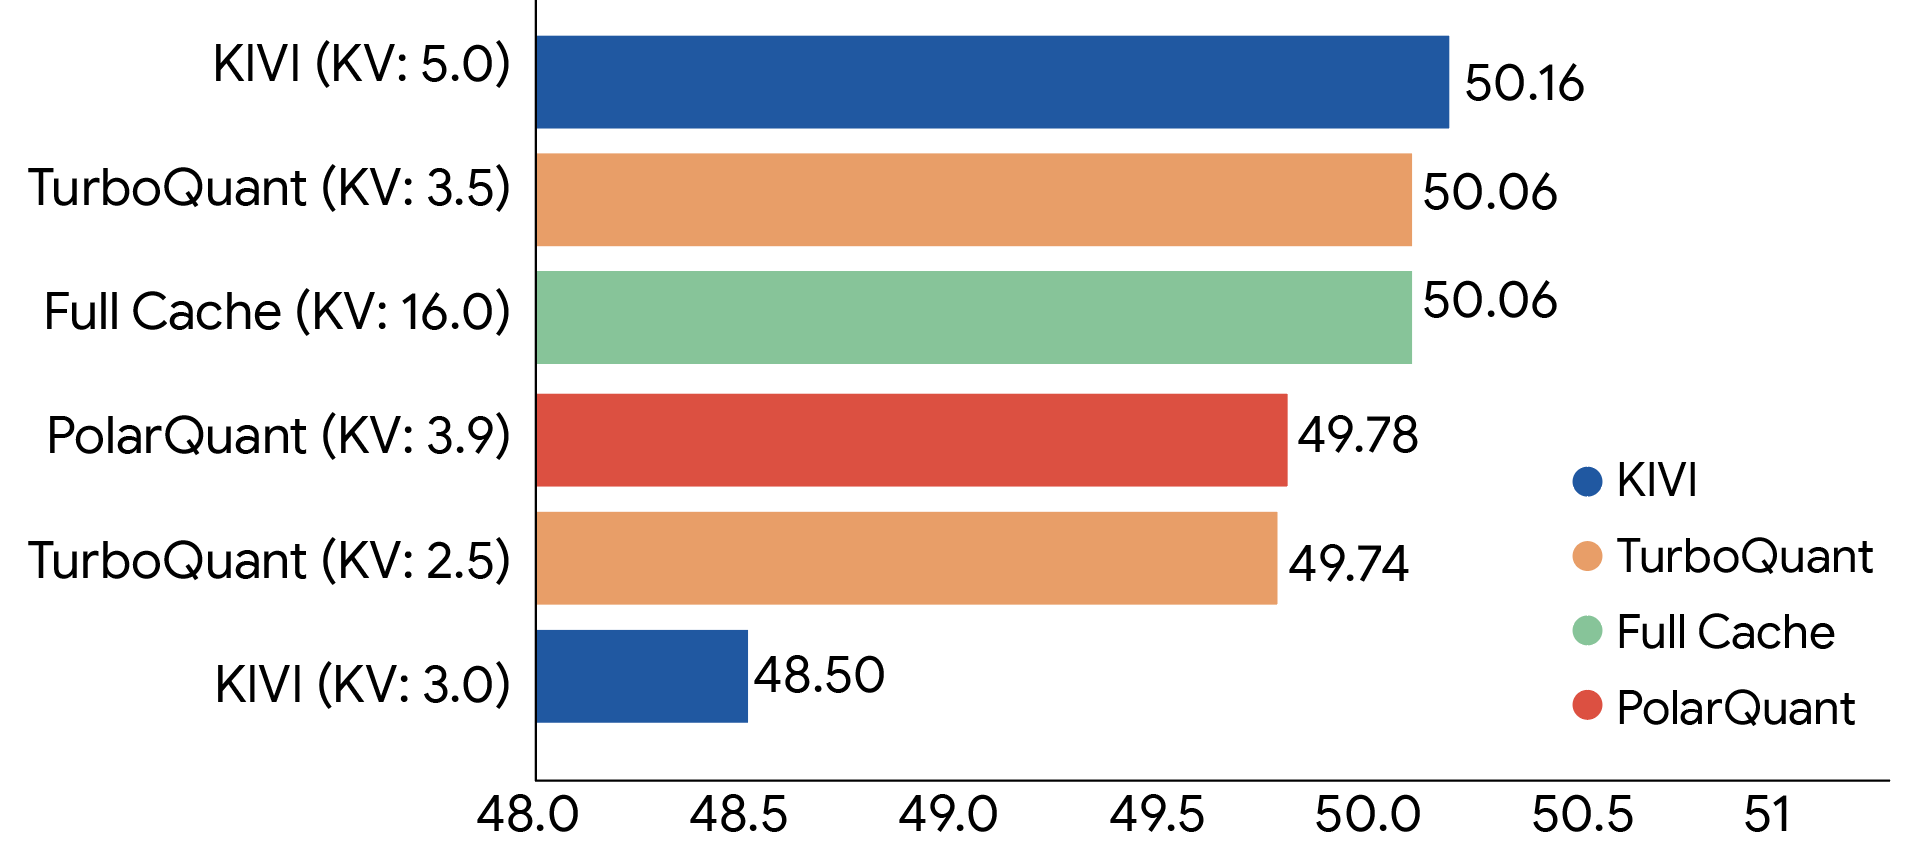
\includegraphics[width=\linewidth,height=0.82\textheight,keepaspectratio]{assets/New-Lecture-Inference_Optimisation/google_research_turboquant_longbench_llama.png}\\[0.35em]
  {\scriptsize Aggregated scores across LongBench-style tasks (QA, code, summarization) for TurboQuant, PolarQuant, and KIVI baselines; bit-widths in brackets. Reference: Google Research Blog.}
\end{frame}

\begin{frame}{TurboQuant: Experiments and Results}
  \centering
  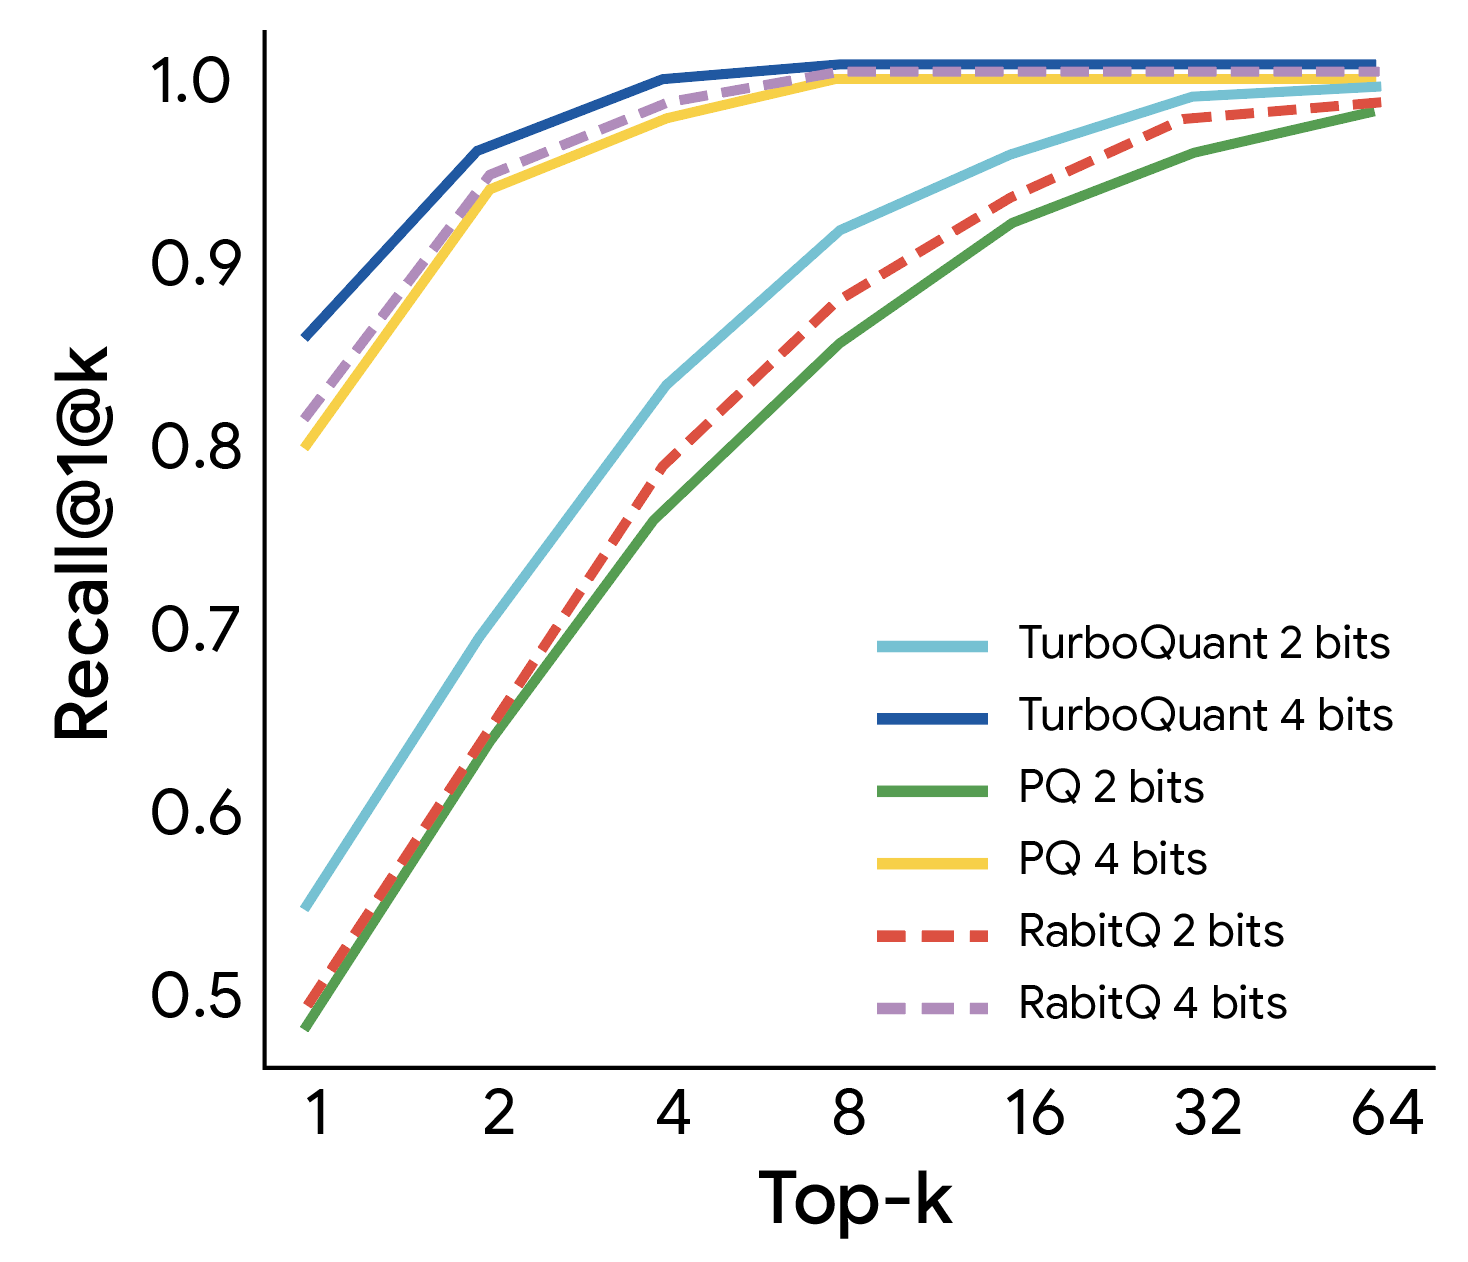
\includegraphics[width=\linewidth,height=0.82\textheight,keepaspectratio]{assets/New-Lecture-Inference_Optimisation/google_research_turboquant_glove_recall.png}\\[0.35em]
  {\scriptsize \textbf{1@$k$ recall} on GloVe ($d{=}200$): TurboQuant vs.\ PQ / RabitQ-style baselines. Reference: Google Research Blog.}
\end{frame}
